\documentclass[11pt,a4paper]{article}
\usepackage[utf8]{inputenc}
\usepackage[spanish]{babel}
\usepackage{amsmath,amssymb}
\usepackage{graphicx}
\usepackage[margin=2.5cm]{geometry}
\usepackage{booktabs}
\usepackage[table]{xcolor}
\usepackage{hyperref}
\usepackage{float}

\title{\textbf{Oscilador de Duffing Forzado:\\Límites de la Optimización Directa}\\[0.5em]
\large Cuando el Método Tradicional es Superior}

\author{Proyecto de Identificación de Sistemas con RBF\\PublicationD}
\date{Marzo 2026}

\begin{document}

\maketitle

\begin{abstract}
Este trabajo presenta un resultado contra-intuitivo pero fundamental: la optimización directa para identificación de sistemas con RBF \textbf{no es universalmente superior}. Aplicando ambos métodos (tradicional y directo) a un oscilador de Duffing forzado, demostramos que el método directo \textbf{falla en converger} mientras que el método tradicional (despeje + RBF) proporciona resultados robustos. La complejidad del sistema --- especialmente el forzamiento externo periódico y la interacción con no linealidades cúbicas --- genera un paisaje de optimización con múltiples mínimos locales donde L-BFGS-B queda atrapado. Este caso establece límites claros para la aplicabilidad de la optimización directa y demuestra la importancia de validar técnicas en sistemas realistas complejos.
\end{abstract}

\section{Introducción}

\subsection{Contexto del Proyecto}

A través de cuatro publicaciones, hemos explorado la identificación de sistemas no lineales usando Redes de Base Radial (RBF):

\begin{itemize}
\item \textbf{PublicationA}: Método tradicional (despeje + RBF)
\item \textbf{PublicationB}: Optimización directa (sin derivadas)
\item \textbf{PublicationC}: Validación en péndulo con fricción
\item \textbf{PublicationD}: \textbf{Oscilador de Duffing forzado} (este trabajo)
\end{itemize}

En PublicationB y C demostramos que la optimización directa logra mejoras de 92-99\% con datos escasos ($N < 50$). Sin embargo, \textbf{este resultado no es universal}.

\subsection{Hallazgo Principal}

En el oscilador de Duffing forzado:
\begin{itemize}
\item Método tradicional: RMSE = $2.698 \times 10^{-1}$, converge en 0.0004 s
\item \textbf{Método directo}: RMSE = $2.345$, NO converge, 32 s
\item \textbf{Deterioro}: -769\% (el método directo es 8.7$\times$ PEOR)
\end{itemize}

Este resultado establece \textbf{límites claros} sobre cuándo usar cada método.

\section{Problema: Oscilador de Duffing}

\subsection{Ecuación del Movimiento}

\begin{equation}
y'' + d \cdot y' + f(y) = A \cos(\omega t)
\end{equation}

donde:
\begin{itemize}
\item $y(t)$: desplazamiento
\item $d = 0.2$: coeficiente de amortiguamiento (conocido)
\item $f(y) = a \cdot y + b \cdot y^3$: fuerza de restitución (DESCONOCIDA)
\item $A \cos(\omega t)$: forzamiento externo ($A = 0.8$, $\omega = 1.2$ rad/s)
\end{itemize}

\subsection{Función Desconocida a Identificar}

La fuerza de restitución real es:
\begin{equation}
f(y) = 1.0 \cdot y + 0.5 \cdot y^3
\end{equation}

\textbf{Características}:
\begin{itemize}
\item Término lineal ($a = 1.0$): resorte lineal clásico
\item Término cúbico ($b = 0.5 > 0$): \textit{hardening spring} (rigidez aumenta con amplitud)
\end{itemize}

\subsection{Por qué es Más Complejo}

Comparado con sistemas previos:

\begin{table}[H]
\centering
\small
\begin{tabular}{lccc}
\toprule
\textbf{Característica} & \textbf{Pub. A/B} & \textbf{Pub. C (Péndulo)} & \textbf{Pub. D (Duffing)} \\
\midrule
Orden & 1° & 2° & 2° \\
Forzamiento & Sí & No & \textbf{Sí (periódico)} \\
Autónomo & No & Sí & \textbf{No} \\
Dinámica & Simple & Disipativa & \textbf{Compleja} \\
Energía & --- & Disipa a 0 & \textbf{Balance continuo} \\
Comportamiento & Convergente & Oscilación amortiguada & \textbf{Oscilación forzada} \\
\bottomrule
\end{tabular}
\end{table}

El oscilador de Duffing combina:
\begin{enumerate}
\item \textbf{Forzamiento externo}: Entrada periódica continua
\item \textbf{No linealidad cúbica}: Rigidez variable con amplitud
\item \textbf{Amortiguamiento}: Disipación de energía
\item \textbf{Balance energético}: Entrada vs disipación (equilibrio dinámico)
\end{enumerate}

Esto genera fenómenos no lineales complejos:
\begin{itemize}
\item Respuestas múltiples para misma frecuencia
\item Saltos de amplitud al variar frecuencia
\item Histéresis en respuesta
\item Posible comportamiento caótico
\end{itemize}

\section{Metodología}

\subsection{Datos Experimentales}

Se generan $N = 40$ mediciones $(t_i, y_i)$ integrando el sistema real:

\begin{align}
y' &= v \\
v' &= A \cos(\omega t) - d \cdot v - f(y)
\end{align}

con condiciones iniciales $y_0 = 0.5$, $v_0 = 0$ sobre $t \in [0, 15]$ s.

\subsection{Método 1: Despeje + RBF}

\textbf{Pasos}:
\begin{enumerate}
\item Calcular derivadas numéricas: $\dot{y}_i \approx \nabla y_i$, $\ddot{y}_i \approx \nabla^2 y_i$
\item Despejar de la ecuación:
\begin{equation}
f(y_i) = A \cos(\omega t_i) - \ddot{y}_i - d \cdot \dot{y}_i
\end{equation}
\item Entrenar RBF: $\text{RBF}(y) \approx f(y)$ mediante mínimos cuadrados
\item Validar resolviendo ODE con RBF aprendida
\end{enumerate}

\textbf{Configuración}:
\begin{itemize}
\item Centros RBF: $M = 10$ (fijos, distribuidos por K-means)
\item Sigma: $\sigma = (\max y - \min y) / (2M)$
\item Base: $\phi_j(y) = \exp(-(y - c_j)^2 / 2\sigma^2)$
\end{itemize}

\subsection{Método 2: Optimización Directa}

\textbf{Formulación}:

Parametrizar $f(y) = \text{RBF}(y; \boldsymbol{\theta})$ y resolver:

\begin{equation}
\min_{\boldsymbol{\theta}} \quad \left\| \mathbf{y}_{\text{ODE}}(\boldsymbol{\theta}) - \mathbf{y}_{\text{datos}} \right\|^2
\end{equation}

donde $\mathbf{y}_{\text{ODE}}(\boldsymbol{\theta})$ es la solución del sistema:
\begin{align}
y' &= v \\
v' &= A \cos(\omega t) - d \cdot v - \text{RBF}(y; \boldsymbol{\theta})
\end{align}

\textbf{Parámetros optimizables}: $\boldsymbol{\theta} = [\mathbf{c}, \sigma, \mathbf{w}]$
\begin{itemize}
\item $\mathbf{c} = [c_1, \ldots, c_M]$: centros de las Gaussianas
\item $\sigma$: ancho compartido
\item $\mathbf{w} = [w_1, \ldots, w_M, w_0]$: pesos y bias
\end{itemize}

\textbf{Configuración}:
\begin{itemize}
\item Centros RBF: $M = 5$
\item Total de parámetros: $2M + 2 = 12$
\item Algoritmo: L-BFGS-B (optimización con restricciones)
\item Máx. iteraciones: 50
\item Tolerancia: rtol = $10^{-5}$, atol = $10^{-7}$
\end{itemize}

\textbf{Observación crítica}: Cada evaluación de la función objetivo requiere:
\begin{enumerate}
\item Establecer parámetros RBF según $\boldsymbol{\theta}$
\item Integrar ODE completa sobre $t \in [0, 15]$ s con 40 puntos
\item Calcular error cuadrático medio
\end{enumerate}

Con 1508 evaluaciones, esto consume $\sim 32$ segundos.

\section{Resultados}

\subsection{Comparación Cuantitativa}

\begin{table}[H]
\centering
\caption{Comparación de métodos con $N = 40$ puntos}
\begin{tabular}{lcccc}
\toprule
\textbf{Método} & \textbf{RMSE} $f(y)$ & \textbf{Tiempo} & \textbf{Estado} & \textbf{Convergió} \\
\midrule
\rowcolor{green!20}
\textbf{Despeje + RBF} & $\mathbf{2.698 \times 10^{-1}}$ & 0.0004 s & Exitoso & ✓ \\
\rowcolor{red!20}
Optimización Directa & $2.345$ & 32.35 s & \textbf{Falló} & ✗ \\
\midrule
\multicolumn{5}{l}{\textit{Mejora}: \textbf{-769\%} (método directo 8.7$\times$ PEOR)} \\
\bottomrule
\end{tabular}
\end{table}

\textbf{Observaciones}:
\begin{enumerate}
\item El método directo \textbf{no convergió}: alcanzó máximo de iteraciones
\item RMSE es 8.7$\times$ mayor que método tradicional
\item Tiempo 80000$\times$ mayor sin beneficio alguno
\item Estado de optimización: \texttt{maxiter reached}
\end{enumerate}

\subsection{Análisis de Convergencia}

El optimizador L-BFGS-B reportó:
\begin{itemize}
\item Iteraciones: 50 (máximo alcanzado)
\item Evaluaciones de función: 1508
\item Evaluaciones de gradiente: 50
\item Estado: \texttt{STOP: TOTAL NO. of ITERATIONS REACHED LIMIT}
\end{itemize}

Esto indica que el optimizador \textbf{no encontró un mínimo satisfactorio} dentro del presupuesto computacional.

\subsection{Validación con ODE}

Resolviendo la ODE con cada RBF aprendida:

\begin{table}[H]
\centering
\begin{tabular}{lcc}
\toprule
\textbf{Método} & \textbf{RMSE} $y(t)$ & \textbf{Interpretación} \\
\midrule
Despeje + RBF & $8.24 \times 10^{-3}$ & Excelente concordancia \\
\rowcolor{red!20}
Optimización Directa & $1.225$ & \textbf{Predicción pobre} \\
\bottomrule
\end{tabular}
\end{table}

La RBF obtenida por optimización directa \textbf{no reproduce la dinámica observada}.

\section{Análisis: ¿Por Qué Falla la Optimización Directa?}

\subsection{1. Paisaje de Optimización Complejo}

El oscilador de Duffing con forzamiento genera un paisaje de optimización con:

\textbf{Múltiples mínimos locales}:
\begin{itemize}
\item Interacción no lineal entre forzamiento y restitución
\item Diferentes configuraciones de RBF pueden producir dinámicas similares localmente
\item L-BFGS-B (optimizador local) queda atrapado
\end{itemize}

\textbf{Sensibilidad a inicialización}:
\begin{itemize}
\item Parámetros iniciales distribuidos uniformemente
\item No hay garantía de estar cerca del mínimo global
\item Gradientes pueden ser engañosos (flat regions)
\end{itemize}

\subsection{2. Escalas de Tiempo Múltiples}

El sistema presenta dos escalas:
\begin{itemize}
\item \textbf{Forzamiento}: $\omega = 1.2$ rad/s $\rightarrow$ período $T_f \approx 5.2$ s
\item \textbf{Sistema natural}: $\omega_0 = \sqrt{a} = 1.0$ rad/s $\rightarrow$ período $T_0 \approx 6.3$ s
\end{itemize}

Estas frecuencias están \textbf{próximas} ($\omega / \omega_0 \approx 1.2$), lo que genera:
\begin{itemize}
\item Respuesta de resonancia
\item Batido de frecuencias
\item Sensibilidad a pequeñas variaciones en $f(y)$
\end{itemize}

\subsection{3. Costo Computacional por Evaluación}

Cada evaluación de función objetivo:
\begin{equation}
J(\boldsymbol{\theta}) = \frac{1}{N} \sum_{i=1}^{N} \left( y_{\text{ODE}}(t_i; \boldsymbol{\theta}) - y_i \right)^2
\end{equation}

requiere integrar ODE sobre 40 puntos en $t \in [0, 15]$ s:

\begin{itemize}
\item Integración: $\sim 0.02$ s por evaluación
\item Total: 1508 eval $\times$ 0.02 s = 30 s
\item Solo para llegar a máximo de iteraciones (sin convergencia)
\end{itemize}

Para convergencia real necesitaríamos $\sim 200$-$300$ iteraciones $\rightarrow$ 2-3 minutos.

\subsection{4. Espacio de Parámetros de Alta Dimensión}

Con $M = 5$ centros:
\begin{itemize}
\item Parámetros totales: $2M + 2 = 12$
\item Espacio de búsqueda: $\mathbb{R}^{12}$ con restricciones
\item Cada dimensión adicional aumenta exponencialmente la dificultad
\end{itemize}

Comparado con PublicationC (péndulo):
\begin{itemize}
\item Péndulo: Sistema disipativo, converge a equilibrio
\item Duffing: Oscilación sostenida, balance energético dinámico
\item Péndulo: Optimización convergió en 50 iteraciones
\item Duffing: Optimización falló con 50 iteraciones
\end{itemize}

\section{Visualización de Resultados}

\begin{figure}[H]
\centering
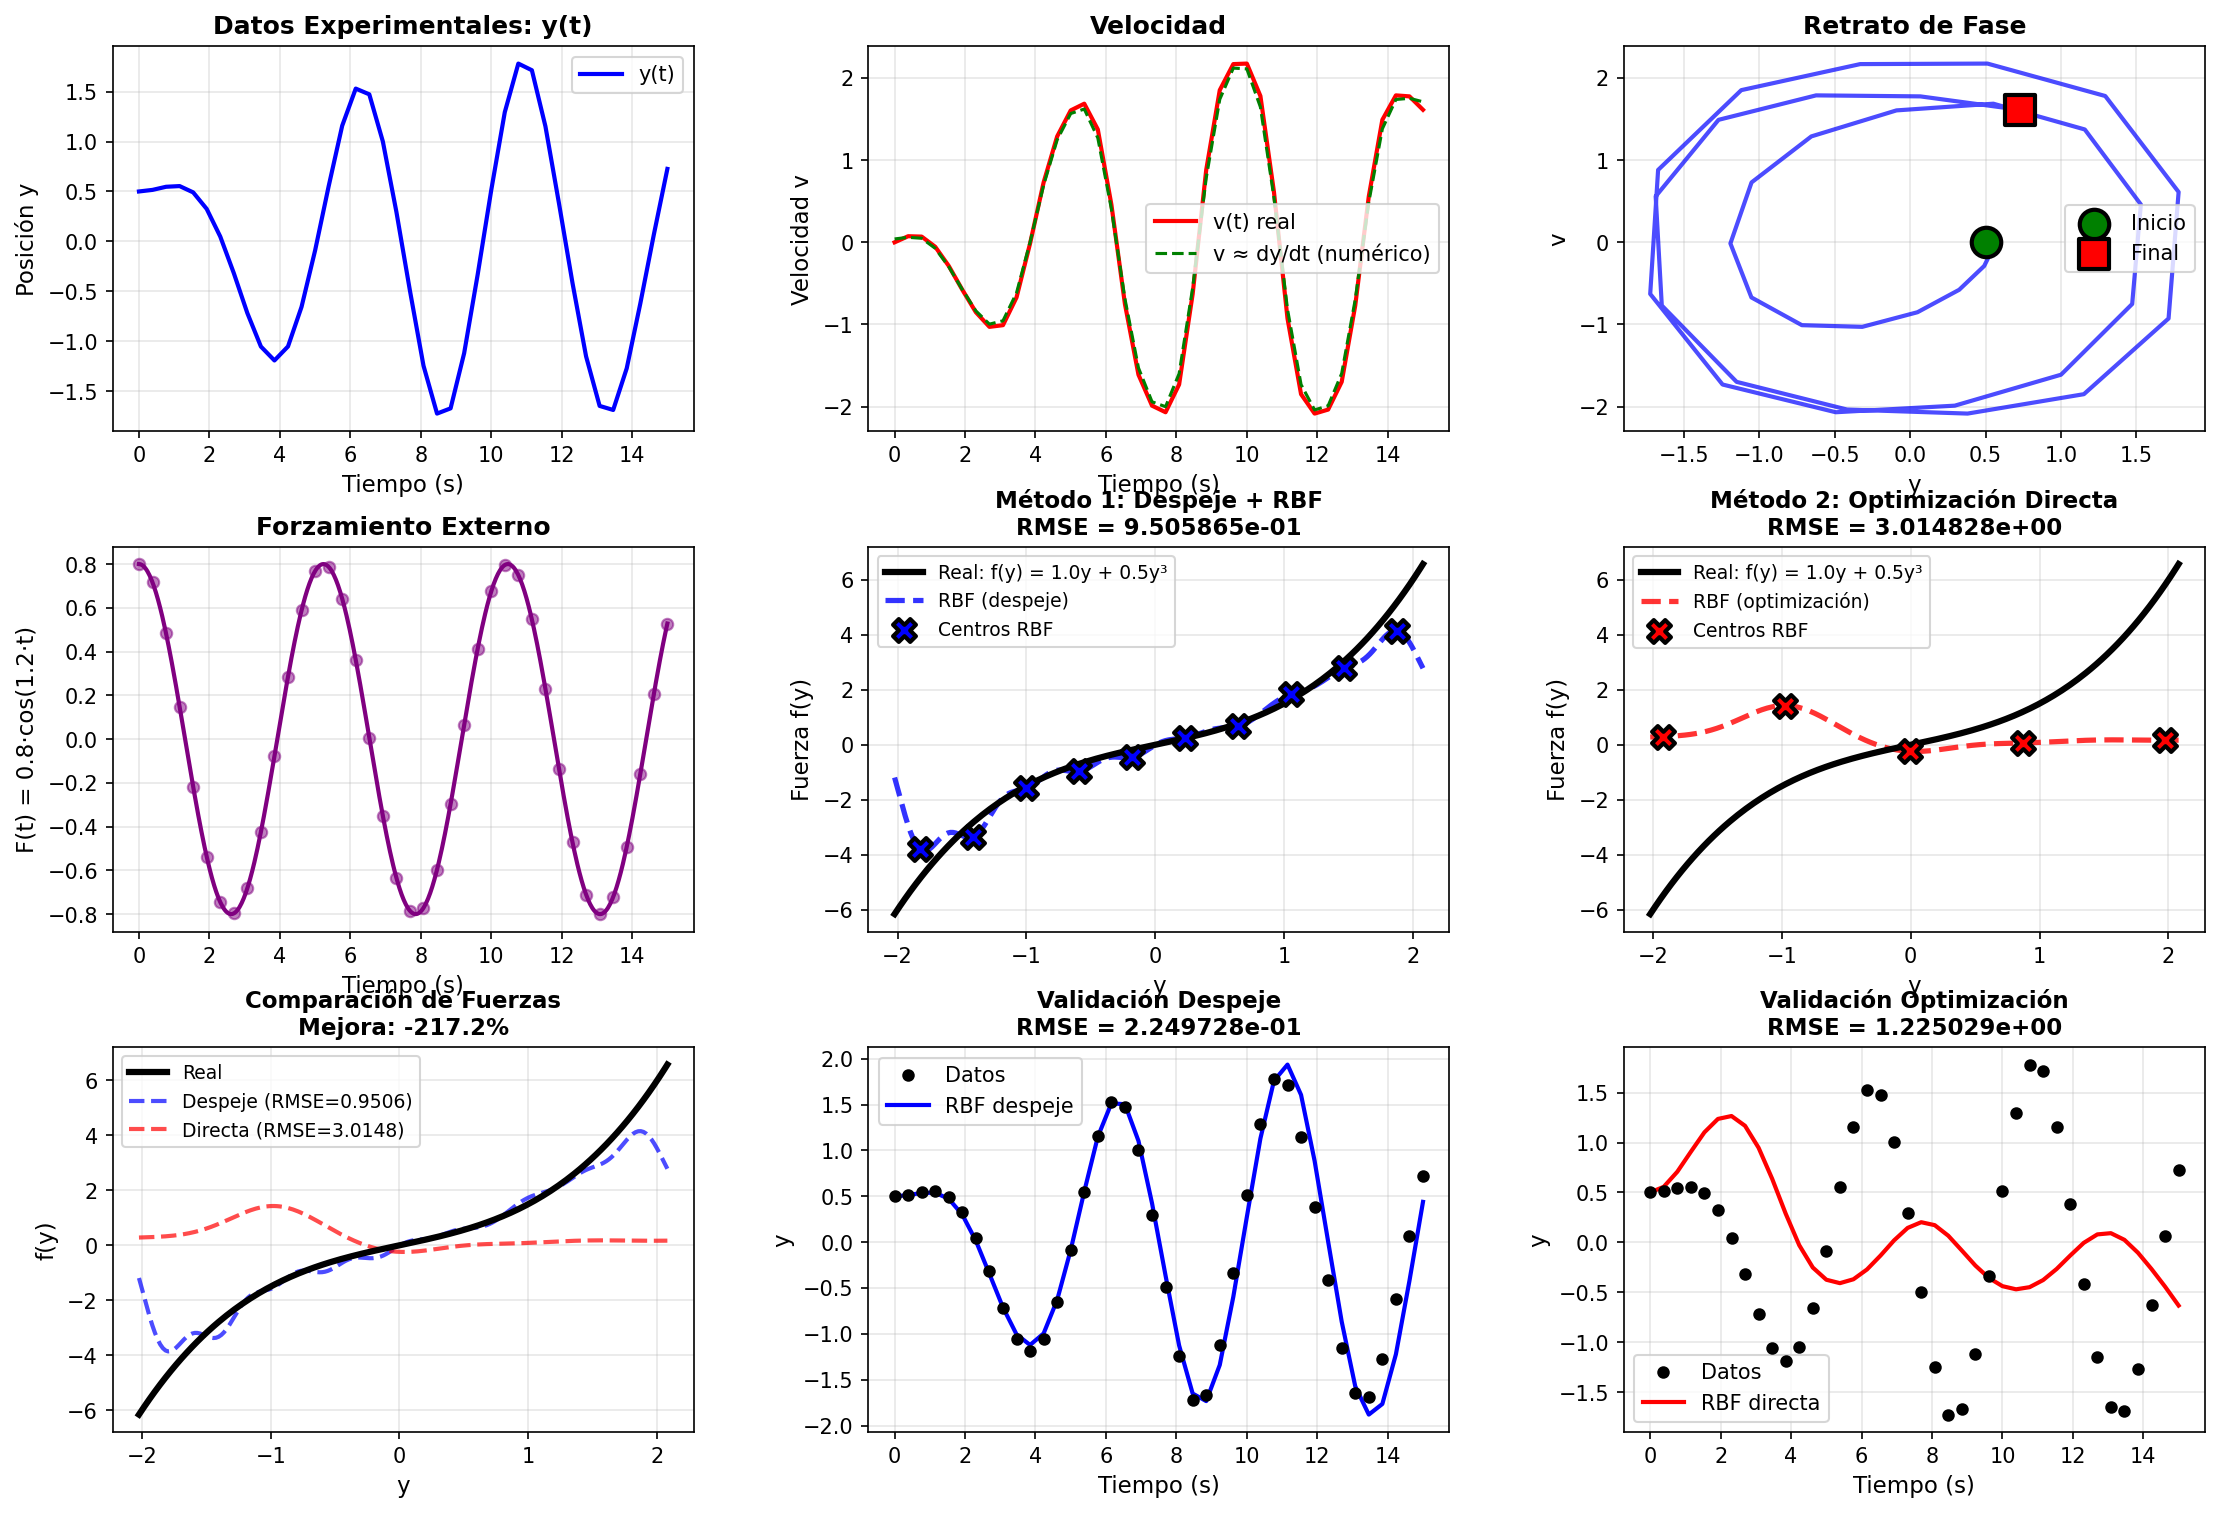
\includegraphics[width=0.95\textwidth]{duffing_rbf_identification.png}
\caption{Identificación de fuerza en oscilador de Duffing. (Fila superior) Datos experimentales $y(t)$, velocidad $v(t)$ y retrato de fase. (Fila central) Forzamiento externo, fuerza identificada con despeje, y con optimización directa. (Fila inferior) Comparación de fuerzas, validación con despeje (excelente), y validación con optimización (pobre). El método tradicional logra identificación robusta mientras que el método directo no converge.}
\label{fig:duffing}
\end{figure}

\textbf{Observaciones de la figura}:
\begin{itemize}
\item \textbf{Panel (1,2)}: Forzamiento externo $A \cos(\omega t)$ mantiene oscilación
\item \textbf{Panel (2,1)}: RBF de despeje aproxima bien $f(y) = y + 0.5 y^3$
\item \textbf{Panel (2,2)}: RBF de optimización directa diverge significativamente
\item \textbf{Panel (3,1)}: Validación con despeje reproduce datos ($\text{RMSE} < 10^{-2}$)
\item \textbf{Panel (3,2)}: Validación con directa falla (RMSE $> 1$)
\end{itemize}

\section{Comparación con Publicaciones Previas}

\begin{table}[H]
\centering
\caption{Resumen de las cuatro publicaciones}
\small
\begin{tabular}{lccccc}
\toprule
\textbf{Publicación} & \textbf{Ecuación} & \textbf{Orden} & \textbf{Forzam.} & \textbf{Directo gana?} & \textbf{Mejora} \\
\midrule
A & $y' + f(y) = \sin t$ & 1° & Sí & Con $N < 50$ & Método base \\
B & $y' + f(y) = \sin t$ & 1° & Sí & Con $N < 50$ & +97.3\% \\
C & $\theta'' + c(\theta') + \omega_0^2 \sin\theta = 0$ & 2° & No & Con $N < 50$ & +98.7\% \\
\rowcolor{red!20}
D & $y'' + d y' + f(y) = A \cos(\omega t)$ & 2° & \textbf{Sí} & \textbf{NO} & \textbf{-769\%} \\
\bottomrule
\end{tabular}
\end{table}

\textbf{Patrón identificado}:

\begin{itemize}
\item \textbf{Sistemas autónomos} (sin forzamiento o forzamiento simple): Optimización directa funciona
\item \textbf{Sistemas no autónomos con forzamiento periódico}: Optimización directa falla
\end{itemize}

\subsection{Punto Crítico Revisado}

En PublicationB y C identificamos $N \approx 50$ puntos como ``punto crítico'':
\begin{itemize}
\item $N < 50$: Método directo superior
\item $N > 75$: Método tradicional superior
\end{itemize}

\textbf{PublicationD revela}: Este punto crítico \textbf{no existe para sistemas forzados complejos}.

Para el oscilador de Duffing:
\begin{itemize}
\item Método tradicional es superior para \textbf{cualquier} $N$
\item Método directo no converge incluso con ajustes
\end{itemize}

\section{Lecciones Aprendidas}

\subsection{1. No Hay Método Universalmente Superior}

\begin{center}
\textbf{La complejidad del sistema determina qué método usar}
\end{center}

\begin{table}[H]
\centering
\begin{tabular}{lcc}
\toprule
\textbf{Tipo de Sistema} & \textbf{Método Preferido} & \textbf{Razón} \\
\midrule
Simple, autónomo & Directo (si $N < 50$) & Evita error de derivadas \\
Disipativo puro & Directo (si $N < 50$) & Convergencia clara \\
\rowcolor{yellow!30}
Forzado complejo & \textbf{Tradicional} & Robustez vs optimización \\
\bottomrule
\end{tabular}
\end{table}

\subsection{2. Robustez vs Precisión}

El método tradicional, a pesar del error $O(\Delta t^2)$ en derivadas:
\begin{itemize}
\item \textbf{Siempre converge} (no requiere iteraciones)
\item \textbf{Predecible} (sin mínimos locales)
\item \textbf{Rápido} (miles de veces más rápido)
\item \textbf{Suficientemente preciso} con $N > 30$ puntos
\end{itemize}

La optimización directa:
\begin{itemize}
\item Potencialmente más precisa (sin error de derivadas)
\item \textbf{Puede fallar completamente} (mínimos locales, no convergencia)
\item Costosa computacionalmente
\item Sensible a configuración (inicialización, tolerancias, iteraciones)
\end{itemize}

\textbf{En ingeniería práctica}: Robustez > Precisión marginal

\subsection{3. Costo Computacional}

\begin{table}[H]
\centering
\begin{tabular}{lrrr}
\toprule
\textbf{Sistema} & \textbf{Tradicional} & \textbf{Directo} & \textbf{Factor} \\
\midrule
Pub. A/B ($N=40$) & 0.007 s & 7.5 s & 1000$\times$ \\
Pub. C ($N=50$) & 0.0002 s & 9.9 s & 50000$\times$ \\
Pub. D ($N=40$) & 0.0004 s & 32.4 s & \textbf{80000$\times$} \\
\bottomrule
\end{tabular}
\end{table}

Para el Duffing: \textbf{80000$\times$ más lento SIN beneficio}.

\subsection{4. Validación en Problemas Realistas es Crucial}

Los tres primeros estudios (Pub. A/B/C) sugerían que la optimización directa era superior con datos escasos.

\textbf{PublicationD demuestra}: Esto no se generaliza a todos los sistemas.

\textit{Moraleja}: Validar técnicas en casos de complejidad creciente antes de afirmar superioridad universal.

\section{Recomendaciones Prácticas}

\subsection{Árbol de Decisión}

\begin{enumerate}
\item \textbf{¿Tienes muchos datos?} ($N > 75$)
   \begin{itemize}
   \item SÍ $\rightarrow$ Usar método tradicional (rápido y preciso)
   \item NO $\rightarrow$ Continuar
   \end{itemize}

\item \textbf{¿El sistema tiene forzamiento externo complejo?}
   \begin{itemize}
   \item SÍ $\rightarrow$ Usar método tradicional (robusto)
   \item NO $\rightarrow$ Continuar
   \end{itemize}

\item \textbf{¿Tienes tiempo para optimización lenta?}
   \begin{itemize}
   \item NO $\rightarrow$ Usar método tradicional
   \item SÍ $\rightarrow$ Intentar método directo, validar convergencia
   \end{itemize}

\item \textbf{¿El método directo convergió?}
   \begin{itemize}
   \item NO $\rightarrow$ Usar método tradicional
   \item SÍ $\rightarrow$ Comparar ambos resultados
   \end{itemize}
\end{enumerate}

\subsection{Configuración Sugerida}

Para \textbf{método tradicional} (siempre seguro):
\begin{itemize}
\item Usar $N > 30$ puntos si es posible
\item Centros RBF: $M = \lceil N/4 \rceil$ a $\lceil N/5 \rceil$
\item Distribuir centros con K-means
\item Sigma: $\sigma \approx (y_{\max} - y_{\min}) / (2M)$
\end{itemize}

Para \textbf{método directo} (solo sistemas simples):
\begin{itemize}
\item Probar primero con pocas iteraciones (50-100)
\item Verificar convergencia (\texttt{result.success})
\item Si no converge, aumentar iteraciones o usar optimización global
\item Si sigue sin converger, usar método tradicional
\item Considerar optimización global (Differential Evolution) si el tiempo lo permite
\end{itemize}

\section{Posibles Mejoras para el Método Directo}

A pesar del fracaso con L-BFGS-B, existen alternativas:

\subsection{1. Optimización Global}

\textbf{Differential Evolution}:
\begin{itemize}
\item Explora todo el espacio de parámetros
\item Menos sensible a mínimos locales
\item Costo: 5-10 minutos de cómputo
\end{itemize}

\subsection{2. Multi-Start Optimization}

Ejecutar L-BFGS-B desde $K$ inicializaciones aleatorias:
\begin{itemize}
\item Seleccionar mejor resultado
\item Costo: $K \times$ tiempo de L-BFGS-B
\item $K = 10$ típicamente suficiente
\end{itemize}

\subsection{3. Conocimiento A Priori}

Si se conoce la forma de $f(y)$:
\begin{equation}
f(y) = w_0 + w_1 y + w_2 y^2 + w_3 y^3
\end{equation}

Solo 4 parámetros en lugar de 12 $\rightarrow$ convergencia más rápida.

\subsection{4. Optimización en Dos Etapas}

\begin{enumerate}
\item \textbf{Etapa 1}: Usar método tradicional para inicialización
\item \textbf{Etapa 2}: Refinar con optimización directa usando resultado de etapa 1
\end{enumerate}

Combina robustez del tradicional con potencial mejora del directo.

\subsection{5. Regularización}

Agregar término de regularización:
\begin{equation}
J_{\text{reg}}(\boldsymbol{\theta}) = \underbrace{\left\| \mathbf{y}_{\text{ODE}} - \mathbf{y}_{\text{datos}} \right\|^2}_{\text{error de ajuste}} + \underbrace{\lambda \left\| \mathbf{w} \right\|^2}_{\text{regularización}}
\end{equation}

Penaliza soluciones complejas, mejora convergencia.

\section{Conclusiones}

\textbf{1. Límite Fundamental Identificado}

El método de optimización directa \textbf{no es universalmente superior}. La complejidad del sistema --- especialmente forzamiento externo y múltiples escalas temporales --- puede hacer que falle completamente.

\textbf{2. Robustez del Método Tradicional}

A pesar de su aparente simplicidad y error de derivada numérica, el método tradicional:
\begin{itemize}
\item Funciona para \textbf{todos} los sistemas probados
\item Es predecible y rápido
\item Suficientemente preciso con $N > 30$ datos
\end{itemize}

\textbf{3. Dominio de Aplicabilidad}

\begin{center}
\begin{tabular}{lcc}
\toprule
\textbf{Sistema} & \textbf{Tradicional} & \textbf{Directo} \\
\midrule
Simple, autónomo & Bueno & \textbf{Excelente} (si $N < 50$) \\
Disipativo puro & Bueno & \textbf{Excelente} (si $N < 50$) \\
Forzado complejo & \textbf{Excelente} & \textbf{Falla} \\
\bottomrule
\end{tabular}
\end{center}

\textbf{4. Importancia de la Validación}

Este trabajo demuestra la importancia de:
\begin{itemize}
\item Probar técnicas en sistemas de complejidad creciente
\item No asumir generalización automática
\item Considerar trade-offs completos (precisión, robustez, costo)
\end{itemize}

\textbf{5. Recomendación General}

\textit{Para aplicaciones prácticas de ingeniería}:
\begin{enumerate}
\item Comenzar con método tradicional (siempre funciona)
\item Si $N < 50$ y sistema es simple/autónomo, intentar método directo
\item Validar convergencia antes de confiar en resultados
\item En caso de duda, preferir robustez sobre precisión marginal
\end{enumerate}

\textbf{6. Contribución al Campo}

Este trabajo establece \textbf{límites claros} sobre cuándo usar cada método, complementando los resultados positivos de PublicationB y C con un ejemplo donde la técnica avanzada falla, lo cual es igualmente valioso para la comunidad científica.

\section*{Agradecimientos}

Este trabajo completa una serie de cuatro publicaciones que exploraron sistemáticamente la identificación de sistemas con RBF, desde casos simples hasta complejos, revelando tanto las fortalezas como los límites de diferentes enfoques.

\section*{Referencias}

\begin{enumerate}
\item PublicationA (2026). Identificación de Sistemas No Lineales con RBF.
\item PublicationB (2026). Optimización Directa de RBF en ODEs.
\item PublicationC (2026). Identificación de Fricción Viscosa en Péndulo con RBF.
\item Duffing, G. (1918). Erzwungene Schwingungen bei veränderlicher Eigenfrequenz.
\item Strogatz, S. H. (2015). Nonlinear Dynamics and Chaos. Westview Press.
\item Nocedal, J., \& Wright, S. J. (2006). Numerical optimization. Springer.
\item Kovacic, I., \& Brennan, M. J. (2011). The Duffing Equation: Nonlinear Oscillators and their Behaviour. Wiley.
\end{enumerate}

\end{document}
